\chapter{A rendszer felhasználása}
\label{chap:felhasznalas}

Az előző fejezetben bemutattam, hogyan helyeztem üzembe a rendszert, milyen kísérleti protokollt használtam, és milyen eredményeket kaptam a végső Log-Mel alapú 2D CNN modellel. Ebben a fejezetben már nem a tanítási és mérési oldalt ismétlem meg, hanem azt mutatom be, hogyan használható a rendszer felhasználói szemszögből: mit lát a program indításakor az ember, hogyan működik a valós idejű konzolos visszajelzés, és milyen helyzetekben viselkedik stabilan vagy bizonytalanabbul.

A rendszer jelenlegi formájában nem grafikus alkalmazás, hanem parancssori felismerő eszköz. Ezt tudatos döntésként kezeltem: a célom nem egy látványos felület elkészítése volt, hanem egy gyorsan futtatható, kevés erőforrást igénylő, valós időben reagáló prototípus. Emiatt a felület egyszerű, de a fontos információkat közvetlenül mutatja: az aktuális osztályt, a hozzá tartozó konfidenciát és a többi osztály pillanatnyi valószínűségét.

\section{Az alkalmazás indítása}
\label{sec:inditas}

A telepítési és futtatási előfeltételeket a \ref{sec:uzembehelyezes}.~szakaszban már összefoglaltam. A használat szempontjából a lényeg az, hogy a virtuális környezet aktiválása és a mikrofon kiválasztása után a valós idejű felismerő modul az alábbi paranccsal indítható:

\begin{lstlisting}
python scripts/05a_realtime_recognition.py
\end{lstlisting}

Indításkor a program betölti a kiválasztott Keras modellt, majd megjeleníti a futás közbeni legfontosabb beállításokat. A jelenlegi konfigurációban a scriptben a \texttt{MODEL\_TYPE = "exp\_final"} beállítás aktív, ezért alapértelmezetten az \texttt{exp\_final} modellmappából dolgozik. Ha a \texttt{CHECKPOINT\_NAME} változó nincs kézzel beállítva, akkor a program automatikusan a legfrissebb Log-Mel alapú checkpointot választja ki a \texttt{models/exp\_final/} könyvtárból. Ez kényelmes a mindennapi futtatásnál, de reprodukálható bemutatóhoz természetesen kézzel is megadható egy konkrét checkpointnév.

\begin{figure}[H]
    \centering
    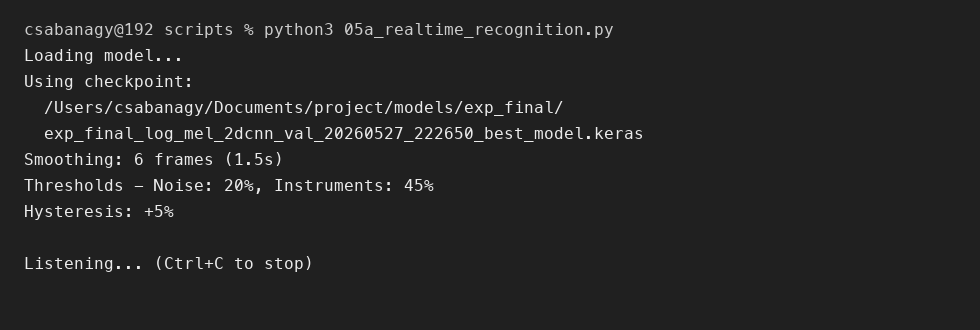
\includegraphics[width=0.75\textwidth]{fig_realtime_setup.png}
    \caption{Konzolos példa az alkalmazás indításakor megjelenő konfigurációs adatokra}
    \label{fig:realtime_setup}
\end{figure}

A \ref{fig:realtime_setup}.~ábra egy tipikus indítási állapotot szemléltet. Itt nem külön mérési eredményről van szó, hanem arról, hogy a program visszajelzi: melyik modellt használja, mekkora simítási ablakot alkalmaz, és milyen konfidenciaküszöbök mellett dönt az aktív osztály megjelenítéséről.

\section{Valós idejű feldolgozás futás közben}
\label{sec:realtime_mukodes}

Az élő felismerés során a program folyamatosan olvassa a mikrofonból érkező hangot. A beérkező jel egy 1 másodperces pufferben gyűlik, majd a rendszer ebből számít Log-Mel spektrogramot. A predikció nem minden egyes hangmintára külön történik, hanem 0,25 másodperces lépésközzel frissül. Ez a gyakorlatban azt jelenti, hogy a kijelzés elég sűrűn változhat ahhoz, hogy élőnek érződjön, de nem minden apró pillanatnyi zaj alapján hoz végleges döntést.

A fontosabb futásidejű paramétereket a \ref{tab:realtime_parameters}.~táblázat foglalja össze.

\begin{table}[H]
\centering
\caption{A valós idejű felismerő modul főbb futásidejű paraméterei}
\label{tab:realtime_parameters}
\begin{tabular}{llp{6.4cm}}
\toprule
\textbf{Paraméter} & \textbf{Érték} & \textbf{Szerep} \\
\midrule
Bemeneti ablak & 1,0 s & Ennyi hangból készül egy Log-Mel spektrogram. \\
Lépésköz & 0,25 s & Ilyen gyakran frissül a predikció. \\
Simítás & 6 predikció & Körülbelül 1,5 másodperces mozgóátlag a stabilabb kijelzésért. \\
Zajküszöb & 20\% & A zaj/csend osztály alacsonyabb küszöbbel is megjelenhet. \\
Hangszerküszöb & 45\% & Új hangszerosztály csak ekkora konfidencia felett vált aktívvá. \\
Hiszterézis & +5\% & Az aktuális osztály kis előnyt kap, hogy a kijelzés ne váltogasson túl gyorsan. \\
\bottomrule
\end{tabular}
\end{table}

A simítás és a hiszterézis nem változtatja meg a neurális háló nyers képességét. Inkább felhasználói oldali stabilizálásként működik. Ha például két hasonló osztály valószínűsége közel van egymáshoz, akkor a kijelzés nem vált át minden apró ingadozásra. Ez különösen fontos a fúvós hangszereknél, ahol a \ref{sec:vegso_teszt}.~szakaszban bemutatott konfúziós mátrix alapján is látható, hogy a nádfúvós és rézfúvós osztályok között a modell gyakrabban bizonytalan.

\section{A parancssori felület felépítése}
\label{sec:cli_dashboard}

A valós idejű visszajelzést egy folyamatosan frissülő terminálsor adja. Ezt a felületet nem részletes grafikus elemzőeszköznek szántam, hanem gyors állapotjelzőnek: futás közben egy pillantással látszódjon, hogy a modell éppen mit tart a legvalószínűbbnek, és mennyire biztos ebben.

A kijelzett sor három fő részből áll:
\begin{enumerate}
    \item \textbf{Konfidenciasáv:} egy 20 karakter hosszú vizuális sáv, amely az aktív osztály simított valószínűségét mutatja.
    \item \textbf{Aktív osztály:} az aktuálisan megjelenített hangszer vagy zaj kategória neve, százalékos konfidenciával.
    \item \textbf{Másodlagos valószínűségek:} a többi osztály rövidített jelölése és pillanatnyi valószínűsége, ami segít észrevenni, ha a modell két osztály között bizonytalan.
\end{enumerate}

A program a terminál egyetlen sorát írja felül folyamatosan, ezért futás közben nem keletkezik hosszú, nehezen olvasható napló. Ez egyszerű megoldás, de élő bemutatónál praktikus: nem kell grafikus ablak, nincs külön vizualizációs szerver, és a program egy átlagos terminálban is használható.

\subsection{Színkódolás és jelölések}

A könnyebb olvashatóság miatt minden osztály saját színt és rövidítést kapott. Ezeket a \ref{tab:ansi_colors}.~táblázat foglalja össze. A színek nem befolyásolják a predikciót, csak a gyorsabb emberi értelmezést segítik.

\begin{table}[H]
\centering
\caption{A parancssori felületen alkalmazott osztályjelölések}
\label{tab:ansi_colors}
\begin{tabular}{llcl}
\toprule
\textbf{Kategória} & \textbf{Terminál színe} & \textbf{Rövidítés} & \textbf{Leírás} \\
\midrule
\texttt{guitar} & Sárga & G & Gitár jellegű pengetős hangok \\
\texttt{piano} & Inverz fekete/fehér & P & Zongora és billentyűs jellegű hangok \\
\texttt{vocal} & Ciánkék & V & Emberi énekhang \\
\texttt{string} & Sötétvörös & S & Vonós hangszerek \\
\texttt{reed} & Narancssárga & R & Nádas fúvós hangszerek \\
\texttt{brass} & Világosbarna & B & Rézfúvós hangszerek \\
\texttt{noise} & Szürke & N & Környezeti zaj vagy csend \\
\bottomrule
\end{tabular}
\end{table}

\section{Működési forgatókönyvek}
\label{sec:forgatokonyvek}

Az alábbi példák azt mutatják meg, hogyan jelenik meg a rendszer kimenete tipikus használati helyzetekben. Ezek nem külön statisztikai mérések, hanem konzolos működési példák. A számszerű modellértékelést az előző fejezet tartalmazza.

\subsection{Csendes vagy zajos szobai környezet}

Alaphelyzetben, amikor nincs aktív hangszeres játék, a rendszernek nem szabad minden apró zörejt hangszerként kezelnie. A végső teszten a zaj osztály bizonyult az egyik legerősebb kategóriának, \(85{,}9\%\)-os F1-score értékkel. Ez a használat során is fontos, mert egy valós idejű felismerő alkalmazás gyakran többet hall csendből, szobazajból és háttérzörejből, mint tényleges hangszerből.

\begin{figure}[H]
    \centering
    
\includegraphics[width=0.7\textwidth]{fig_realtime_noise.png}
    \caption{Konzolos példa zaj vagy csend felismerésekor}
    \label{fig:realtime_noise}
\end{figure}

A \ref{fig:realtime_noise}.~ábrán látható állapotban a \texttt{noise} osztály jelenik meg aktívként. Ilyenkor a felület nem azt állítja, hogy a környezet tökéletesen néma, hanem azt, hogy a modell számára nincs olyan domináns hangszeres mintázat, amely valamelyik hangszerosztályhoz erősebben kötődne.

\subsection{Gitárjáték}

Gitár esetén a modell viselkedése óvatosabban értelmezendő. A végső teszten a gitár precision értéke magas volt (\(88{,}5\%\)), vagyis amikor a modell gitárt jelzett, általában jó döntést hozott. A recall viszont csak \(59{,}0\%\) lett, ami azt mutatja, hogy nem minden valódi gitármintát talált meg gitárként. Ez használat közben úgy jelenhet meg, hogy a gitár stabil felismerése erősen függ a hangszíntől, a játékmódtól és a mikrofonba érkező jel tisztaságától.

\begin{figure}[H]
    \centering
    
\includegraphics[width=0.7\textwidth]{fig_realtime_guitar.png}
    \caption{Konzolos példa gitárként azonosított bemenet esetén}
    \label{fig:realtime_guitar}
\end{figure}

A \ref{fig:realtime_guitar}.~ábra ezért nem általános garancia minden gitárhangra, hanem egy olyan pillanatot mutat, amikor a modell a bemenetet gitárként értelmezte. Ez a különbség fontos: a rendszer használható demóként, de a mérési eredmények alapján nem érdemes úgy kezelni, mint minden gitártípust egyformán biztosan felismerő megoldást.

\subsection{Emberi énekhang}

A vokál osztály a végső teszten kiegyensúlyozottabb eredményt adott, \(75{,}6\%\)-os F1-score-ral. Használat közben ez azért érdekes, mert az emberi hang sokszor nagyon eltérő lehet: beszédszerű, énekelt, halk, erősen formánsos vagy levegős. A modell ennek ellenére több esetben stabilan tudja vokálként értelmezni a bemenetet, főleg akkor, ha a mikrofonba érkező jel tiszta és a háttérzaj nem túl erős.

\begin{figure}[H]
    \centering
    
\includegraphics[width=0.7\textwidth]{fig_realtime_vocal.png}
    \caption{Konzolos példa vokálként azonosított bemenet esetén}
    \label{fig:realtime_vocal}
\end{figure}

A \ref{fig:realtime_vocal}.~ábrán látható visszajelzésnél a másodlagos osztályok értékei is hasznosak: ha például a zaj vagy más hangszerosztály valószínűsége megemelkedik, abból látszik, hogy a modell nem teljesen egyértelmű bemenetet kap.

\subsection{Nádfúvós és rézfúvós bizonytalanság}

A fúvós hangszerek jó példát adnak arra, hogy a rendszer nem csak találatokat, hanem bizonytalanságot is mutat. A végső konfúziós mátrix alapján a rézfúvós osztály több esetben nádfúvósként vagy vonósként jelent meg. Ez a használat során is előfordulhat, különösen akkor, ha a bemenet szaxofonhoz, trombitához vagy más erős felhangszerkezetű fúvós hanghoz hasonlít.

\begin{figure}[H]
    \centering
    
\includegraphics[width=0.7\textwidth]{fig_realtime_reed.png}
    \caption{Konzolos példa nádfúvós jellegű bemenet esetén}
    \label{fig:realtime_reed}
\end{figure}

A \ref{fig:realtime_reed}.~ábrán látható \texttt{reed} kimenet ezért nemcsak egy sikeres felismerési példaként érdekes, hanem azt is szemlélteti, miért volt szükség a simításra és a hiszterézisre. Ezek nélkül a kijelzés könnyebben váltogathatna a fúvós osztályok között, ami felhasználói oldalról zavaróbb lenne, még akkor is, ha a nyers valószínűségek szakmailag értelmezhetők.

\section{Használati korlátok}
\label{sec:hasznalati_korlatok}

A rendszer jelenlegi állapotában működő valós idejű prototípus, de nem általános célú, minden zenei helyzetben megbízható hangszerfelismerő alkalmazás. A legfontosabb korlátok a használat során:

\begin{itemize}
    \item \textbf{Monofón vagy domináns hangszeres bemenetre készült.} Ha egyszerre több hangszer szól, a softmax kimenet miatt a modell akkor is egyetlen fő osztályt választ.
    \item \textbf{A mikrofon és a környezet hatása erős.} A final rendszer már tartalmaz mikrofonos tanítóadatokat, de másik szobában, másik mikrofonnal vagy erős háttérzajban a viselkedés változhat.
    \item \textbf{A hasonló hangszínű osztályok között marad bizonytalanság.} Különösen a fúvós, vonós és egyes gitár/zongora jellegű tranziens hangok okozhatnak tévesztést.
    \item \textbf{A kijelzés simított.} A felhasználói élmény stabilabb, de emiatt a rendszer nem a pillanatnyi nyers predikciót, hanem annak rövid időablakon átlagolt változatát mutatja.
\end{itemize}

Ezeket a korlátokat nem hibaként, hanem a jelenlegi prototípus természetes határaiként kezelem. A rendszer célja az volt, hogy egy saját adatokon tanított, valós időben futtatható hangszerfelismerő folyamatot hozzak létre, amelynek működése és hibái is megfigyelhetők. Ezt a célt a használati tesztek és az előző fejezetben bemutatott mérések alapján sikerült teljesíteni.

\section{Az alkalmazás leállítása}
\label{sec:alkalmazas_leallitasa}

Az élő felismerés a terminálban a \texttt{Ctrl+C} billentyűkombinációval szakítható meg. Ilyenkor a program lezárja a mikrofonbemenetet, felszabadítja az audio streamet, és visszatér a parancssorba. Ez egyszerű, de a fejlesztés és bemutatás során praktikus megoldásnak bizonyult: a rendszer gyorsan indítható, gyorsan leállítható, és nem hagy maga után külön bezárandó ablakokat vagy grafikus folyamatokat.
